%===============================================================
%Template for UPC-TALP based on CTU and modified to match UPC-TALP colors and style  
%The original template from Czech Technical University  % Author: Martin Malý.
% They are defined by new graphical manual - 2017.
% Share and modify as you like. Keep the name of the authors.
% It is forbidden to use the template commercially.
%===============================================================

\documentclass{beamer}
\usepackage[utf8]{inputenc}
%\usepackage{lmodern}

\usepackage{comment}
\usetheme{Madrid}
  \usepackage[maxbibnames=99]{biblatex}
\definecolor{cvut_navy}{HTML}{0065BD}
\definecolor{cvut_blue}{HTML}{6AADE4}
\definecolor{cvut_gray}{HTML}{156570}
\usepackage{biblatex}
%\usepackage{tikz}
%\usepackage{pgfplots}
\usepackage[makeroom]{cancel}
\usepackage{threeparttable}
\usepackage[utf8]{inputenc}
%\usepackage[usenames,dvipsnames]{xcolor}
%\addbibresource{biblatex-examples.bib}
%\setbeamercolor{section in toc}{}
\setbeamercolor{section in toc}{fg=black,bg=yellow} 
\setbeamercolor{alerted text}{fg=cvut_blue}
\usepackage{tikzsymbols}
\usepackage{textcomp}
\usepackage{parskip}
\definecolor{darkblue}{rgb}{0, 0, 0.5} 
\definecolor{babyblue}{rgb}{0.54, 0.81, 0.94}
\usepackage{pgf}
\usepackage{color,soul}
%\usepackage{pythontex} 
\usepackage{tcolorbox}
\tcbuselibrary{skins}
\usepackage{minted}
\usepackage{hyperref}
\usepackage{xcolor,soul}
\definecolor{lightblue}{rgb}{.90,.95,1}
\sethlcolor{lightblue}
\renewcommand<>{\hl}[1]{\only#2{\beameroriginal{\hl}}{#1}}
\setbeamertemplate{page number in head/foot}[framenumber]
%%% attravive box over equestion
\usepackage{empheq}
\usepackage{xcolor}
\definecolor{lightgreen}{HTML}{90EE90}
\newcommand{\boxedeq}[2]{\begin{empheq}[box={\fboxsep=6pt\fbox}]{align}\label{#1}#2\end{empheq}}
\newcommand{\coloredeq}[2]{\begin{empheq}[box=\colorbox{lightgreen}]{align}\label{#1}#2\end{empheq}}
\newcommand{\highlight}[1]{%
  \colorbox{red!40}{$\displaystyle#1$}}
  
  
  \definecolor{babyblue}{rgb}{0.54, 0.81, 0.94}
\definecolor{babypink}{rgb}{0.96, 0.76, 0.76}
\definecolor{blue(ncs)}{rgb}{0.0, 0.53, 0.74}
\definecolor{pistachio}{rgb}{0.58, 0.77, 0.45}
\definecolor{darksalmon}{rgb}{0.91, 0.59, 0.48}
\definecolor{lightsalmonpink}{rgb}{1.0, 0.6, 0.6}
\definecolor{columbiablue}{rgb}{0.61, 0.87, 1.0}
\definecolor{corn}{rgb}{0.98, 0.93, 0.36}
\definecolor{jonquil}{rgb}{0.98, 0.85, 0.37}
\definecolor{bananayellow}{rgb}{1.0, 0.88, 0.21}
\newcommand{\bert}{\ensuremath{%
  \mathchoice{\includegraphics[height=2ex]{Bert-pic-removebg-preview.png}} 
    {\includegraphics[height=2ex]{Bert-pic-removebg-preview.png}}
    {\includegraphics[height=1.5ex]{Bert-pic-removebg-preview.png}}
    {\includegraphics[height=1ex]{Bert-pic-removebg-preview.png}}
}}
  
  
\useoutertheme{infolines}



\usepackage{courier}
%\usepackage{animate}  
\usepackage{expl3}
%\usepackage[listings,theorems]{tcolorbox}



%%%%%%%%%%%%%%%%%%%%%%%%%%%%%%%%%%%%%%%%%%%%%%%%%%%%%%%%%%%%%%%%%%%%%  
%commands for simulating terminal in/output  
%\scroll[<line separator string>]{<width as TeX dim>} 
%                             {<number of lines>}{terminal text line}  
%\clearbuf  %clears line buffer  
%%%%%%%%%%%%%%%%%%%%%%%%%%%%%%%%%%%%%%%%%%%%%%%%%%%%%%%%%%%%%%%%%%%%%  



\newcommand\scroll[4][§§]{
  \seq_set_split:Nnn\g_inputline_seq{#1}{#4}
  \seq_map_inline:Nn\g_inputline_seq{
    \seq_gput_right:Nx\g_linebuffer_seq{##1}
    \int_compare:nT{\seq_count:N\g_linebuffer_seq>#3}{
      \seq_gpop_left:NN\g_linebuffer_seq\dummy
    }
  }
  \fbox{\begin{minipage}[t][#3\baselineskip]{#2}
    \ttfamily
    \seq_map_inline:Nn\g_linebuffer_seq{\mbox{##1}\\}
  \end{minipage}}
}
\newcommand\clearbuf{\seq_gclear:N\g_linebuffer_seq}
\ExplSyntaxOff

\setbeamertemplate{headline}{%
\begin{beamercolorbox}[colsep=1.5pt]{upper separation line head}
\end{beamercolorbox}
\begin{beamercolorbox}{section in head/foot}
    \vskip2pt\insertsectionnavigationhorizontal{\paperwidth}{}{\hskip0pt plus1filll}\vskip2pt
\end{beamercolorbox}%

\begin{beamercolorbox}[colsep=1.5pt]{lower separation line head}
\end{beamercolorbox}
}
\makeatletter
\newcommand\SoulColor{%
  \let\set@color\beamerorig@set@color
  \let\reset@color\beamerorig@reset@color}
\makeatother
\SoulColor
\usepackage{amsmath, bm}
\usepackage{tikz}
\setbeamercovered{dynamic}

\newcommand{\highlightt}[1]{%
  \colorbox{blue!40}{$\displaystyle#1$}}


\newenvironment<>{problock}[1]{%
  \begin{actionenv}#2%
      \def\insertblocktitle{#1}%
      \par%
      \mode<presentation>{%
       % \setbeamercolor{block title}{fg=white,bg=orange!20!black}
        %\setbeamercolor{block title}{fg=white,bg=red!10!black}
        \setbeamercolor{block title}{fg=white,bg=cvut_blue}
       \setbeamercolor{block body}{fg=black,bg=white!50}
       \setbeamercolor{itemize item}{fg=orange!20!black}
       \setbeamertemplate{itemize item}[triangle]
     }%
      \usebeamertemplate{block begin}
    \par\usebeamertemplate{block end}
    \end{actionenv}
    }
    
    \newcommand<>{\uncovergraphics}[2][{}]{
    % Taken from: <https://tex.stackexchange.com/a/354033/95423>
    \begin{tikzpicture}
    \node[anchor=south west,inner sep=0] (B) at (4,0)
        {\includegraphics[#1]{#2}};
    \alt#3{}{%
        \fill [draw=none, fill=background, fill opacity=0.9] (B.north west) -- (B.north east) -- (B.south east) -- (B.south west) -- (B.north west) -- cycle;
    }
    \end{tikzpicture}
}




\newlength\dlf
\newcommand\alignedbox[3][yellow]{
  % #1 = color (optional, defaults to yellow)
  % #2 = before alignment
  % #3 = after alignment
  &
  \begingroup
  \settowidth\dlf{$\displaystyle #2$}
  \addtolength\dlf{\fboxsep+\fboxrule}
  \hspace{-\dlf}
  \fcolorbox{red}{#1}{$\displaystyle #2 #3$}
  \endgroup
}

\usepackage{collcell}
\usepackage{booktabs}
\usepackage{etoolbox}
%\usepackage{remreset}% tiny package containing just the \@removefromreset command
\makeatletter

\usepackage{xcoffins}
\NewCoffin\tablecoffin
\NewDocumentCommand\Vcentre{m}
  {%
    \SetHorizontalCoffin\tablecoffin{#1}%
    \TypesetCoffin\tablecoffin[l,vc]%
  }



\usepackage{pgfpages}

%% Important 
%%% show note or disable note. 
%\setbeameroption{show notes on second screen=right} % Both

\setbeamertemplate{note page}{\pagecolor{gray!5}\insertnote}\usepackage{palatino}



%\setbeamertemplate{footline}{}
%\setbeamertemplate{footline}{}
\usepackage{xcolor}
\usepackage{soul}

\usepackage{etoolbox}
\makeatletter
%\patchcmd{\slideentry}{\ifnum#2>0}{\ifnum2>0}{}{\@error{unable to patch}}% replace the subsection number test with a test that always returns true
\makeatother

\setbeamercolor*{palette primary}{bg=cvut_navy,fg=gray!20!white}
\setbeamercolor*{palette secondary}{bg=cvut_navy,fg=gray!20!white} % no color
%\setbeamercolor*{palette secondary}{bg=cvut_navy,fg=cvut_navy}
%\setbeamercolor*{palette secondary}{bg=cvut_blue,fg=white}
\setbeamercolor*{palette tertiary}{parent=palette primary} % color of the top and date
\setbeamercolor*{palette quaternary}{fg=cvut_navy,bg=gray!5!white}
\setbeamercolor*{sidebar}{fg=cvut_navy,bg=gray!15!white}
\usepackage[first=0,last=9]{lcg}
\newcommand{\ra}{\rand0.\arabic{rand}}
\usepackage{color, colortbl}
\usepackage{stackengine,tikz}
\usepackage{transparent}
\usepackage{pgfpages}
%\usepackage{graphicx}% http://ctan.org/pkg/graphicx
\usepackage{booktabs}% http://ctan.org/pkg/booktabs
%\setbeameroption{show notes}
\colorlet{Gray}{gray!30}




    
\newcommand*{\MinNumber}{0}%
%\newcommand*{\MaxNumber}{100}%
\newcommand*{\MaxNumber}{0.4}%
\definecolor{bubblegum}{rgb}{0.99, 0.76, 0.8}
\newcommand{\ApplyGradient}[1]{%
  \pgfmathsetmacro{\PercentColor}{100.0*(#1-\MinNumber)/(\MaxNumber-\MinNumber)}%
  %\textcolor{black!\PercentColor}{#1}
  \edef\x{\noexpand\cellcolor{babyblue!\PercentColor}}\x\textcolor{black}{#1}%
}
\newcolumntype{R}{>{\collectcell\ApplyGradient}{c}<{\endcollectcell}}

%\setbeameroption{show notes on second screen=right}
\setbeamercolor{titlelike}{parent=palette primary}
\setbeamercolor{frametitle}{parent=palette primary}

\setbeamercolor{B}{bg=red!30,fg=black}


\setbeamertemplate{section in toc}[default]
\setbeamercolor{itemize item }{fg=blue}
\setbeamertemplate{itemize item}[circle]

\setbeamercolor*{separation line}{}
\setbeamercolor*{fine separation line}{}

\setbeamertemplate{navigation symbols}{} 
\setbeamertemplate{caption}{\raggedright\insertcaption\par}

%\setbeamercolor*{block title example}{fg=blue!50,bg= blue!10}

%\setbeamercolor*{block title example}{fg=white,bg= cvut_navy}
\setbeamercolor*{block title example}{fg=white,bg=purple!75!black}
\setbeamercolor*{block body example}{fg= black, bg= white}


\setbeamercolor{itemize item}{fg=cvut_navy} % all frames will have red bullets
\setbeamercolor{block title}{bg=red!30,fg=black}
\setbeamertemplate{subsection in toc}[subsections numbered]


\usepackage{eqnarray,amsmath}
\usepackage{amsfonts}
\usepackage{amssymb}
\usefonttheme{professionalfonts}
\usepackage{graphicx}
\usepackage{booktabs} 
\usepackage{bm}
\usepackage{mathtools}
\usepackage[utf8]{inputenc}
\usepackage[T1]{fontenc}
\usepackage{lmodern} 
\usepackage{booktabs}


%\setbeamercolor{block title}{fg=darkred,bg=structure.fg!10!bg!10!bg}
%\setbeamercolor{block body}{use=block title,bg=block title.bg}
\definecolor{NormalBlue}{RGB}{200,200,255}
%\setbeamercolor{block title}{bg=NormalBlue}yellow
\setbeamercolor{block title}{fg=black, bg=yellow}
\setbeamercolor{block2}{use=structure,fg=white,bg=purple!75!black}
% definice makra
\def\bq{\mbox{\kern.1ex\protect\raisebox{-1.3ex}[0pt][0pt]{''}\kern-.1ex}}
\def\eq{\mbox{\kern-.1ex``\kern.1ex}}
\def\ifundefined#1{\expandafter\ifx\csname#1\endcsname\relax }%
\ifundefined{uv}%
        \gdef\uv#1{\bq #1\eq}
\fi


%====================================================
%========== DEFINITION OF AUTHORS ETC...=============
%====================================================
\author[TP 1 - MD]{Julio Cesar da Silva Rodrigues}
\institute[]{Universidade Federal de São João del-rei \\ Curso de Ciência da Computação\\
\vspace{0.5cm}

\includegraphics[height=1.5cm]{Images/LogoUFSJ.PNG}
\vspace{2mm} \\  
%Dr. Marina \\ 
\vspace{2mm}}
\title[]{Detecção de URLs Maliciosas}


  \date[18 de Abril de 2023]{\small{Trabalho Prático 1 - Mineração de Dados} \\ \vspace{0.2cm} \small{18 de Abril de 2023}}
%====================================================
%========== BEGINNING OF DOCUMENT ===================
%====================================================


\begin{document}



\begin{frame}[plain]
%\transboxin

	\titlepage
	\begin{center}%
	%\vspace{-2mm}
	%\tableofcontents{current}
  		
  		%\includegraphics[height=1cm]{darkblue-talp-logo.pdf}
  		%\includegraphics[height=1.5cm]{upclogo.pdf}
		%\includegraphics[height=1.1cm]{files/IRIS.png}
		%\includegraphics[height=1.3cm]{files/logo_iri2.png}https://www.overleaf.com/project/5bed4779c7eea31291e7e8b2#Navigation27
	%\includegraphics[height=1.3cm]{files/IBT.png}
		%\includegraphics[height=1.3cm]{files/biocev-logo-CMYK-horizontal.pdf}
	\end{center}
%\note[item]{you  note here}
\end{frame}


%\logo{\includegraphics[height=1cm]{files/TALP.png}}
%\logo{\includegraphics[height=0.6cm]{darkblue-logo.pdf}}
%\logo{\includegraphics[height=0.5cm]{darkblue-logo.pdf}}



\begin{frame}[plain]{Conteúdo}
\tableofcontents[]
\note[item]{note here }
\end{frame}

\section{Introdução}

\begin{frame}[plain]{Conteúdo} 
     \tableofcontents[currentsection]
\end{frame}

\begin{frame}[noframenumbering]{Tecnologias Utilizadas}

\begin{itemize}
    \item Python 3;
    \item Machine Learning e Manipulação de Dados:
    \begin{enumerate}
        \item scikit-learn;
        \item xgboost;
        \item pandas.
    \end{enumerate}
    \item Visualização dos Dados:
    \begin{enumerate}
        \item Matplotlib;
        \item seaborn.
    \end{enumerate}
\end{itemize}

\end{frame}

\begin{frame}[noframenumbering]{Base de Dados}

\begin{itemize}
    \item URLs Maliciosas:
    \begin{enumerate}
        \item Um atributo;
        \item Uma classe com quatro valores distintos;
        \item Mais de 650 mil instâncias;
        \item Disponível em: \url{https://www.kaggle.com/datasets/sid321axn/malicious-urls-dataset}.
    \end{enumerate}
    \item Objetivos Principais:
    \begin{enumerate}
        \item Criação de Atributos;
        \item Observar como cada novo atributo criado impacta na classificação.
    \end{enumerate}
\end{itemize}

\end{frame}

\begin{frame}[noframenumbering]{Base de Dados}

\begin{figure}[H]
    \centering
    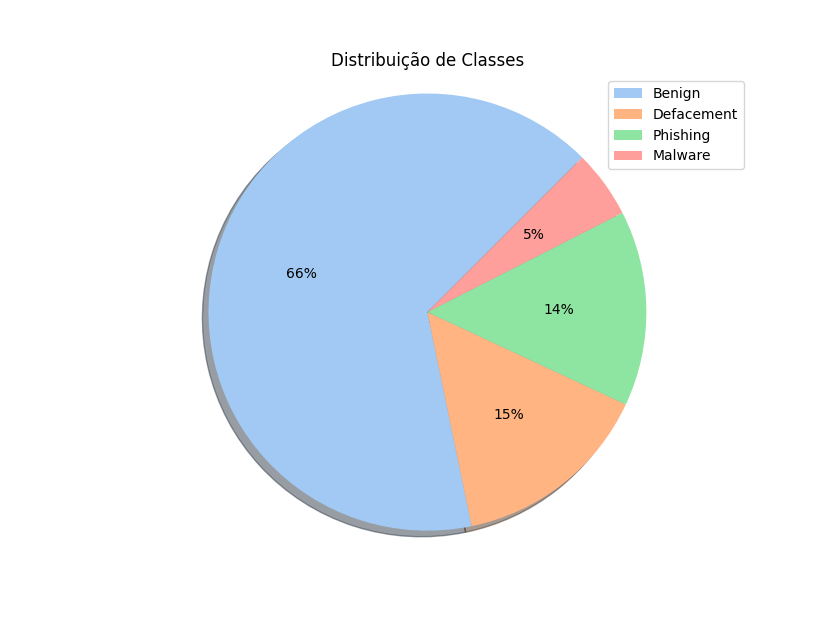
\includegraphics[width=0.9\textwidth]{Beamer/Images/Figure_1.png}
    \label{fig:exampleFig1}
\end{figure}

\end{frame}

\section{Feature Engineering}

\begin{frame}[plain]{Conteúdo} 
     \tableofcontents[currentsection]
\end{frame}

\begin{frame}[noframenumbering]{Análise Léxica}

\begin{figure}[H]
    \centering
    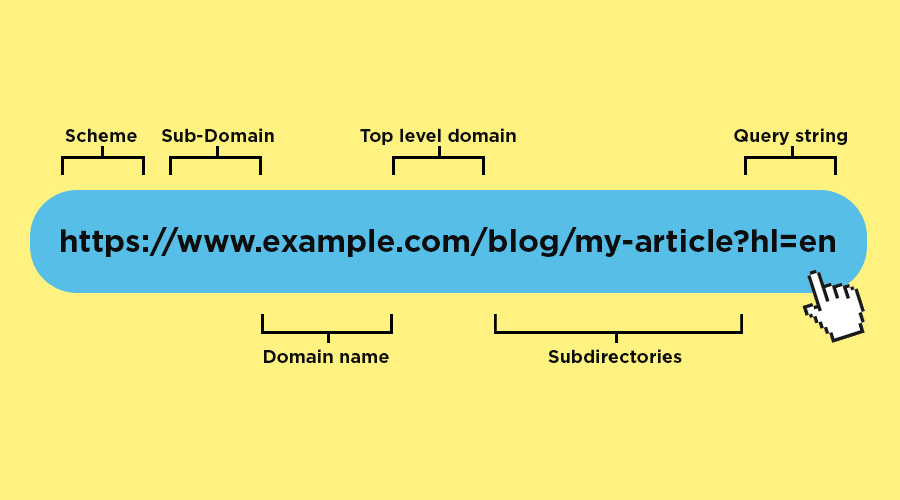
\includegraphics[width=0.9\textwidth]{Beamer/Images/Diagram-of-a-URL.jpg}
    \label{fig:exampleFig2}
\end{figure}

\end{frame}

\begin{frame}[noframenumbering]{Protocolo de Comunicação}

\begin{itemize}
    \item Grande potencial para influenciar na classificação;
    \item Protocolos das URLs presentes na base são distribuídos em:
    \begin{enumerate}
        \item HTTPS;
        \item HTTP;
        \item Não Especificado.
    \end{enumerate}
    \item Somente 2,4\% das URLs utilizam HTTPS (explícito);
    \item 85,7\% das URLs HTTPS são maliciosas (\emph{phishing} e \emph{malware});
    \item Todas as URLs de \emph{defacement} utilizam HTTP.
\end{itemize}

\end{frame}

\begin{frame}[noframenumbering]{Protocolo de Comunicação}

\begin{figure}[H]
    \centering
    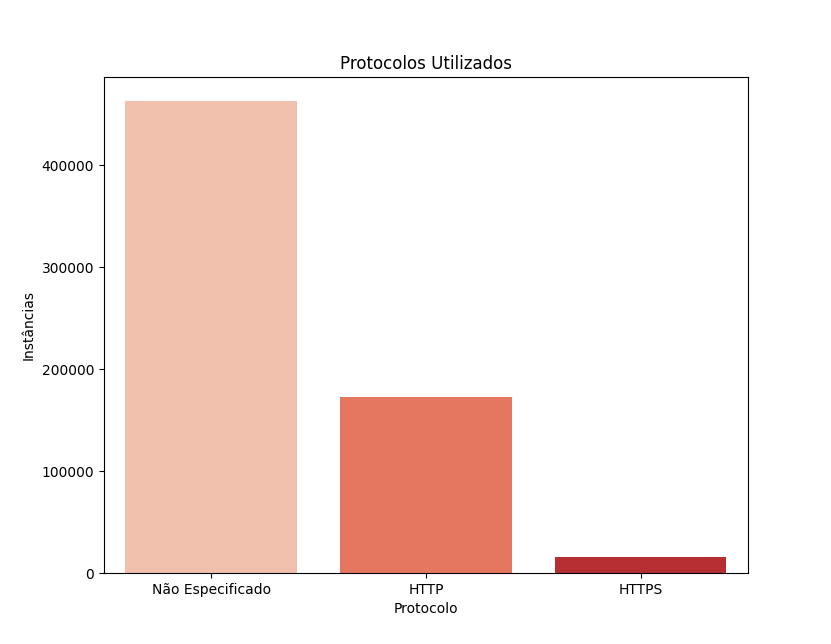
\includegraphics[width=0.8\textwidth]{Beamer/Images/Figure_2.png}
    \label{fig:exampleFig3}
\end{figure}

\end{frame}

\begin{frame}[noframenumbering]{Comprimento de URLs}

\begin{itemize}
    \item Apresentaram ligeiras disparidades entre as classes;
    \item URLs de \emph{defacement} são, em média, 50\% maiores que URLs seguras;
    \item URLs de \emph{phishing} são, em média, 25\% menores que URLs seguras;
    \item URLs HTTPS e HTTP são, em média, de 63\% a 72\% maiores que as de protocolo não explícito.
\end{itemize}

\end{frame}

\begin{frame}[noframenumbering]{Comprimento das URLs}

\begin{figure}[H]
    \centering
    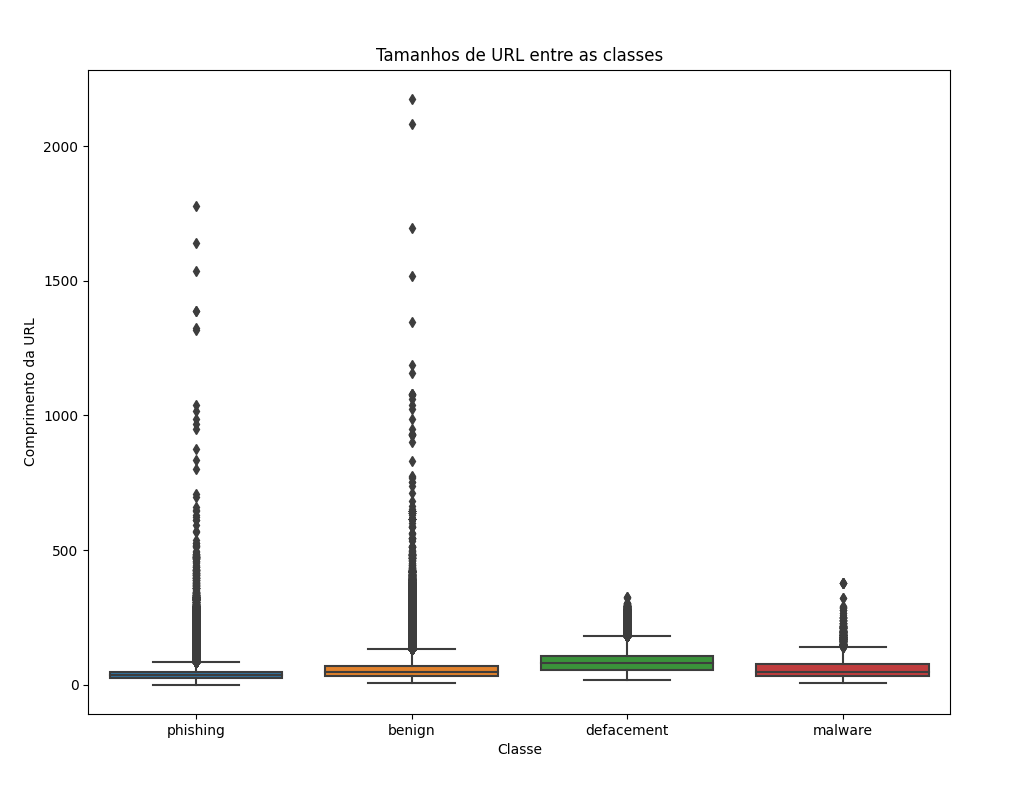
\includegraphics[width=0.8\textwidth]{Beamer/Images/Figure_6.png}
    \label{fig:exampleFig4}
\end{figure}

\end{frame}

\begin{frame}[noframenumbering]{Comprimento das URLs}
\begin{itemize}
    \item Equal-Frequency Binning
\end{itemize}
\begin{figure}[H]
    \centering
    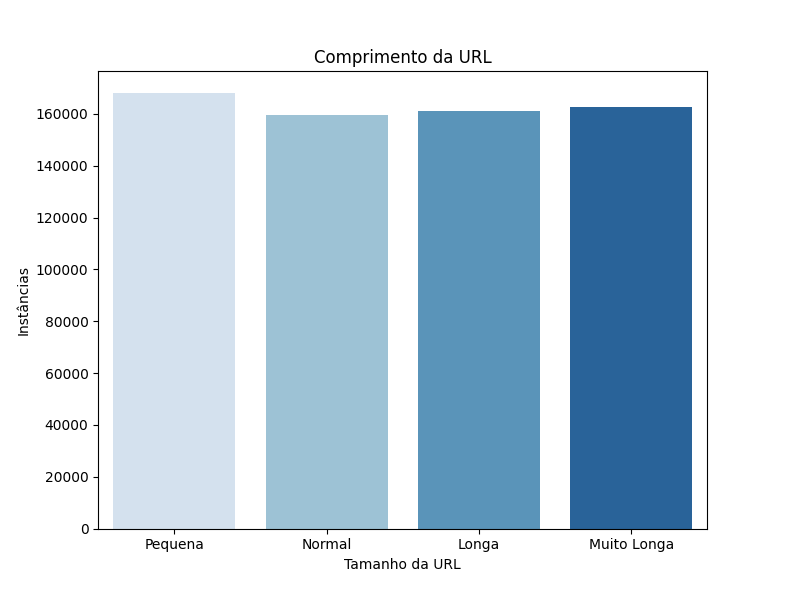
\includegraphics[width=0.75\textwidth]{Beamer/Images/Figure_3.png}
    \label{fig:exampleFig5}
\end{figure}
\end{frame}

\begin{frame}[noframenumbering]{Tamanho do Primeiro Diretório e Quantidade de Dígitos}

\begin{itemize}
    \item Tamanho do primeiro diretório de URLs de \emph{malware} é, em média, o dobro de URLs seguras;
    \item Tamanho do primeiro diretório de URLs de \emph{phishing} é, em média, 25\% menores que de URLs seguras;
    \item URLs de \emph{malware} possuem, em média, mais que o dobro de dígitos de URLs seguras;
    \item URLs de \emph{phishing} possuem, em média, 35\% menos dígitos que URLs seguras.
\end{itemize}

\end{frame}

\begin{frame}[noframenumbering]{Palavras Suspeitas}
\begin{itemize}
    \item Foco em destacar URLs de \emph{phishing};
    \item Impacto muito abaixo do esperado.
\end{itemize}

\begin{figure}[H]
    \centering
    \fbox{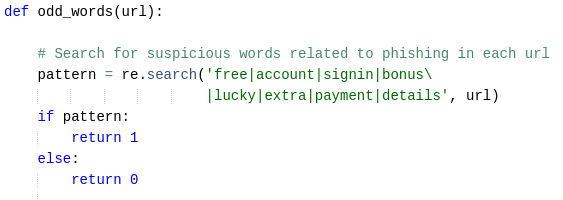
\includegraphics[width=0.8\linewidth]{Beamer/Images/sus.png}}
    \label{fig:exampleFig6}
\end{figure}

\end{frame}

\section{Análise}

\begin{frame}[plain]{Conteúdo} 
     \tableofcontents[currentsection]
\end{frame}

\begin{frame}[noframenumbering]{Ganho de Informação}

\begin{figure}[H]
    \centering
    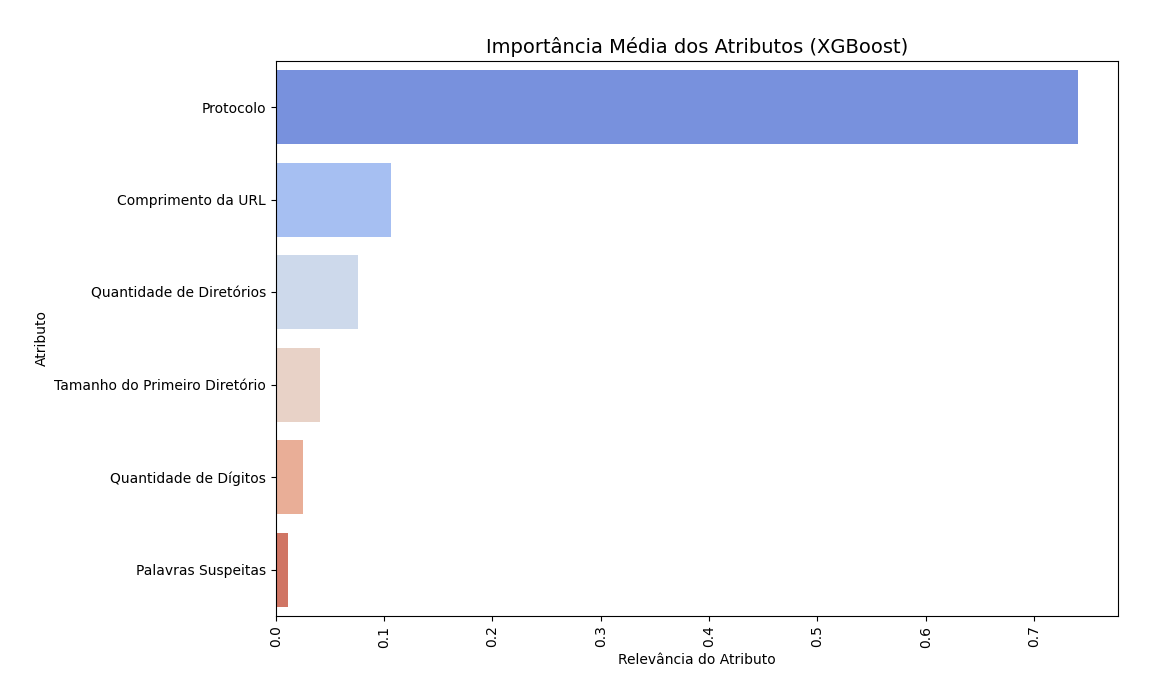
\includegraphics[width=1\textwidth]{Beamer/Images/Figure_4.png}
    \label{fig:exampleFig7}
\end{figure}

\end{frame}

\begin{frame}[noframenumbering]{Ganho de Informação}

\begin{figure}[H]
    \centering
    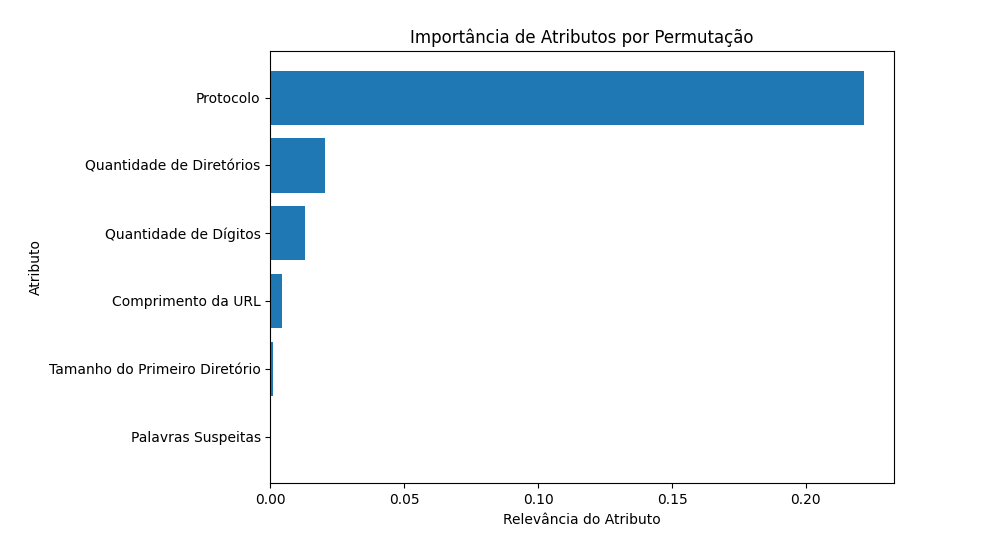
\includegraphics[width=1\textwidth]{Beamer/Images/Figure_5.png}
    \label{fig:exampleFig8}
\end{figure}

\end{frame}

\begin{frame}
	\frametitle{Testes Incrementais}	
%\begin{itemize}





%\end{itemize}
\begin{block}{}
\begin{table}
\centering

\resizebox{\columnwidth}{!}{
\begin{tabular}{|c|c|c|c|c|}

%\begin{tabularx}{\columnwidth}{|lcccc|}
\hline 
 
\multicolumn{5}{|c|}{XGBoost}\\ 
\hline 
\rowcolor{Gray}

Class & Precision & Recall & F1-Score & Support\\
 \hline 
 %\rowcolor{Gray}
%\multicolumn{5}{|c|}{Dictionary} \\ 
% \hline 
Benign & 0.90 & 0.98 & 0.94 & 85621\\   %\hdashline
Defacement & 0.91 & 0.95 & 0.92 & 19292\\   %\hdashline
Phishing & 0.94 & 0.84 & 0.89 & 6504\\   %\hdashline
Malware & 0.85 & 0.51 & 0.64 & 18822\\   %\hdashline
  \hline 
Accuracy &  &  & 0.90 & 130239\\   %\hdashline
Macro Avg & 0.90 & 0.82 & 0.85 & 130239\\   %\hdashline
Weighted Avg & 0.90 & 0.90 & 0.89 & 130239\\   %\hdashline


\end{tabular}
}
%\end{tabularx}
%\label{se:Dic}
\end{table}
\end{block}
\note[item]{.}

\end{frame}

\begin{frame}[noframenumbering]{Matriz de Confusão}

\begin{figure}[H]
    \centering
    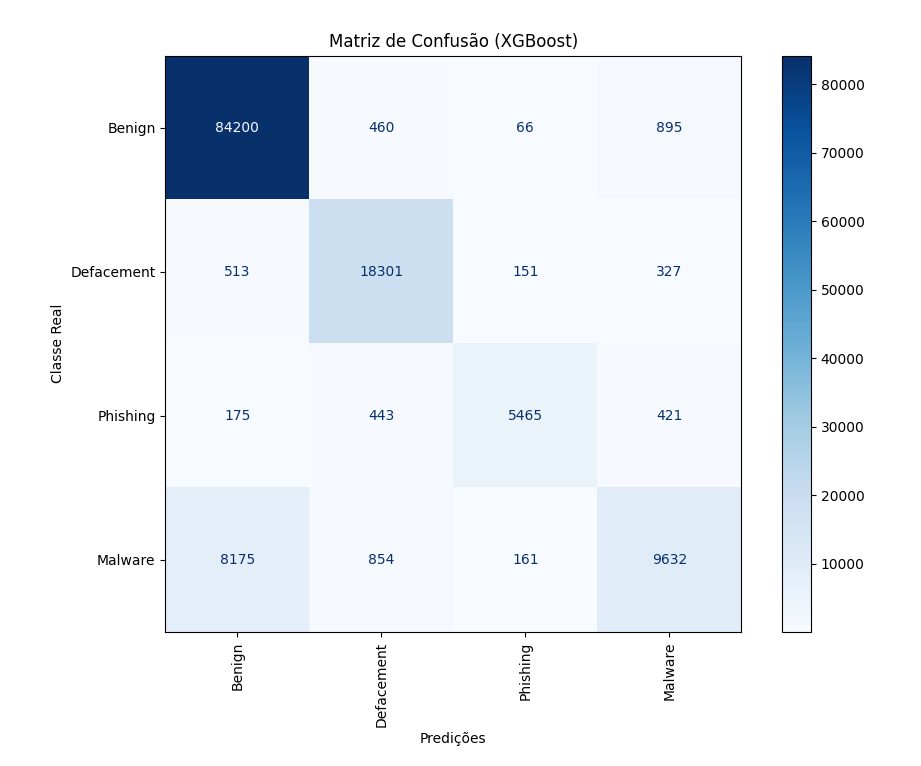
\includegraphics[width=0.75\textwidth]{Beamer/Images/Figure_7.png}
    \label{fig:exampleFig9}
\end{figure}

\end{frame}

\section{Resultados}

\begin{frame}[plain]{Conteúdo} 
     \tableofcontents[currentsection]
\end{frame}

\begin{frame}[noframenumbering]{Modelos de Machine Learning}

\begin{itemize}
    \item Regressão Logística;
    \item XGBoost;
    \item Validação Cruzada (\emph{k-fold}):
    \begin{enumerate}
        \item 10 partes;
        \item Amostragem estratificada;
        \item Métrica \emph{Macro F1}.
    \end{enumerate}
\end{itemize}

\end{frame}

\begin{frame}
	\frametitle{Comparativo de Modelos}	
%\begin{itemize}





%\end{itemize}
\begin{block}{}
\begin{table}
\centering

\resizebox{\columnwidth}{!}{
\begin{tabular}{|c|c|c|}

%\begin{tabularx}{\columnwidth}{|lcccc|}
\hline 
 
\multicolumn{3}{|c|}{Macro F1}\\ 
\hline 
\rowcolor{Gray}

 Modelo & Média  & Desvio Padrão\\
 \hline 
 %\rowcolor{Gray}
%\multicolumn{5}{|c|}{Dictionary} \\ 
% \hline 
Regressão Logística & 0.4343240025832924 & 0.0014418608790156475\\   %\hdashline
XGBoost & 0.8218246353658317 & 0.001907892449405127\\  %\hdashline 
  \hline 


\end{tabular}
}
%\end{tabularx}
%\label{se:Dic}
\end{table}
\end{block}
\note[item]{.}

\begin{itemize}
    \item Calculada para cada uma das classes;
    \item Não leva em conta possível desbalanceamento presente na base de dados;
    \item XGBoost exige mais processamento, mas entregou resultados melhores;
    \item Ainda há grande margem para melhorias.
\end{itemize}
\end{frame}

\section{Conclusão}

\begin{frame}[plain]{Conteúdo} 
     \tableofcontents[currentsection]
\end{frame}

\begin{frame}
	\frametitle{Próximos Passos}	

    \begin{block}{}
    
        \begin{itemize}
            \item Construção de novos atributos;
        \end{itemize}
    
    \end{block}
    
    \begin{block}<0>
    
        \begin{itemize}   
            \item Expandir análises:\\
            \begin{enumerate}
                \item Atributos relacionados à conteúdo;
                \item Atributos relacionados à rede.
            \end{enumerate}
        \end{itemize}
   
    \end{block}
    
    \vspace{0.1cm}
\end{frame}

\begin{frame}
	\frametitle{Próximos Passos}	

    \begin{block}{}
    
        \begin{itemize}
            \item Construção de novos atributos;
        \end{itemize}
    
    \end{block}
    
    \begin{block}{}
    
        \begin{itemize}   
            \item Expandir análises:\\
            \begin{enumerate}
                \item Atributos relacionados à conteúdo;
                \item Atributos relacionados à rede.
            \end{enumerate}
        \end{itemize}
   
    \end{block}
    
    \vspace{0.1cm}
\end{frame}

\begin{frame}
	\frametitle{Próximos Passos}	

    \begin{block}{}
    
        \begin{itemize}
            \item União de classes pode favorecer os modelos;
        \end{itemize}
    
    \end{block}

    \begin{alertblock}{Extração de Classes}
        \{Defacement, Phishing, Malware\} \rightarrow \{\text{Malicious}\}
    \end{alertblock}
    
    \begin{block}<0>
    
        \begin{itemize}   
            \item Balanceamento da base de dados:\\
            \begin{enumerate}
                \item Oversampling;
                \item Instance Selection.
            \end{enumerate}
        \end{itemize}
   
    \end{block}

    \begin{block}<0>
    
        \begin{itemize}
            \item Ajuste fino dos hiperparâmetros dos modelos.
        \end{itemize}
    
    \end{block}
    
    \vspace{0.1cm}
\end{frame}

\begin{frame}
	\frametitle{Próximos Passos}	

    \begin{block}{}
    
        \begin{itemize}
            \item União de classes pode favorecer os modelos;
        \end{itemize}
    
    \end{block}

    \begin{alertblock}{Extração de Classes}
        \{Defacement, Phishing, Malware\} \rightarrow \{\text{Malicious}\}
    \end{alertblock}
    
    \begin{block}{}
    
        \begin{itemize}   
            \item Balanceamento da base de dados:\\
            \begin{enumerate}
                \item Oversampling;
                \item Instance Selection.
            \end{enumerate}
        \end{itemize}
   
    \end{block}

    \begin{block}<0>
    
        \begin{itemize}
            \item Ajuste fino dos hiperparâmetros dos modelos.
        \end{itemize}
    
    \end{block}
    
    \vspace{0.1cm}
\end{frame}

\begin{frame}
	\frametitle{Próximos Passos}	

    \begin{block}{}
    
        \begin{itemize}
            \item União de classes pode favorecer os modelos;
        \end{itemize}
    
    \end{block}

    \begin{alertblock}{Extração de Classes}
        \{Defacement, Phishing, Malware\} \rightarrow \{\text{Malicious}\}
    \end{alertblock}
    
    \begin{block}{}
    
        \begin{itemize}   
            \item Balanceamento da base de dados:\\
            \begin{enumerate}
                \item Oversampling;
                \item Instance Selection.
            \end{enumerate}
        \end{itemize}
   
    \end{block}

    \begin{block}{}
    
        \begin{itemize}
            \item Ajuste fino dos hiperparâmetros dos modelos.
        \end{itemize}
    
    \end{block}
    
    \vspace{0.1cm}
\end{frame}

 \end{document}
% =============================================================
% =========================== END =============================
% =============================================================


